\documentclass[a4paper,10pt,fleqn]{article}

\usepackage{layout}

\newboolean{STANDALONE}
\setboolean{STANDALONE}{false}

\newboolean{EMBED}
\setboolean{EMBED}{false}


\setboolean{STANDALONE}{true}

\newcommand{\BrushlessPath}{src}
\newcommand{\BIBLIOGRAPHY}{src/BLDC_Source}
\newcommand{\DasAndereTeam}{T27}
\newcommand{\BLDCTeams}{T27 und T32}
\newcommand{\BLDCcollab}{Dieses Kapitel ist eine Zusammenarbeit der Gruppen \BLDCTeams. }

\begin{document}
	\begin{titlepage}

\begin{center}

% Oberer Teil der Titelseite:
%\includegraphics[width=0.15\textwidth]{./logo}\\[1cm]    
\textsc{\LARGE Produktentwicklung 1}\\[1.5cm]

\textsc{\Large Hochschule Luzern\\
    ~\\
    Technik \& Architektur}\\[0.5cm]

\vfill{}

% Title
\newcommand{\HRule}{\rule{\linewidth}{0.5mm}}
\HRule \\[0.4cm]
{   \Huge \bfseries Brushless DC Treiber\\
        ~\\
        \large Konzeptbeschreibung}\\[0.4cm]

\HRule \\[1.5cm]

% Author and supervisor
\begin{minipage}{0.4\textwidth}
    \begin{flushleft} \large
        \emph{Autoren:}\\
        Yves \textsc{Studer}\\
        Daniel \textsc{Winz}\\
        Ervin \textsc{Mazlagi\'c}\\
    \end{flushleft}
\end{minipage}
\hfill
\begin{minipage}{0.4\textwidth}
    \begin{flushright} \large
        \emph{Projektgruppe:} \\
        PREN-ET
    \end{flushright}
\end{minipage}

\vfill{}
\vfill{}
\vfill{}

% Unterer Teil der Seite
{\large Horw\\ \today}

\end{center}

\end{titlepage}

	\tableofcontents
	\newpage
	\ifSTANDALONE
\section{Hardware}
\fi
\ifEMBED
\subsection{Hardware}
\fi
Die Elektrotechnik-Studierenden aus mehreren Gruppen haben sich
zusammengeschlossen um gemeinsame Probleme anzugehen. Dabei handelt es sich
um die Ansteuerung, die benötigte Hard- und Software um Motoren anzusteuern
und gegebenenfalls zu regeln. In diesem Zusammenschluss wurde drei Gruppen
gebildet, um Lösungen für DC-, Stepper- und Brushless-Motoren auszuarbeiten.
Die Idee besteht darin, dass nicht jede Gruppe für dasselbe Problem wo
möglich denselben Lösungsansatz verfolgt, sondern die Ressourcen kombiniert,
Synergien nutzt um eine bessere Lösung zu erarbeiten. Auf diese Weise kann
das Team übergreifende Arbeiten im Rahmen der \enquote{PREN} erlernt und
geübt werden. Somit wird Idee der Interdisziplinarität im erweiterten Sinn
Rechnung getragen. Die Gruppen und deren Mitglieder sind in der Tabelle 
\ref{tab:pren-et-overview} aufgeführt.
\begin{table}[h!]
	\centering
	\begin{tabular}{l l}
		Projekt		& Team \\
		\hline
		DC Motoren	& 39 \\
		Schrittmotor	& 27, 38 \\
		BLDC Motor	& 27, 32 \\
	\end{tabular}
	\caption{Übersicht der PREN-ET Projektgruppen}
	\label{tab:pren-et-overview}
\end{table}

	\subsection{Brushless Motoransteuerung}
Dieses Kapitel wurde in Zusammenarbeit mit der Gruppe \DasAndereTeam erstellt. 
\subsubsection{Theorie der Ansteuerung}
\begin{wrapfigure}{r}{0.50\textwidth}
	\includegraphics[scale=0.45]{\BrushlessPath/Bilder/ZeitlicheHallSensorAnsteuerung.jpg}
	\caption[Zeitliche Darstellung der Ansteuerung mit Hall-Sensoren]{Zeitliche Darstellung der Ansteuerung mit Hall-Sensoren \cite{AppNote:BrushlessuC}}
	\centering
    \label{abb:ZeitlicheAnsteuerungBrushlessMotor}
\end{wrapfigure}
Brushless-Motoren sind Synchron-Drehstrom-Motoren. Das heisst, sie werden mittels eines kontinuierlichen Drehfeld in Bewegung gesetzt. Dabei ist darauf zu achten, dass der Läufer dem Drehfeld synchron folgen kann, daher der Name. Falls der Läufer dem Drehfeld aus irgend einem Grund nicht folgen kann, so wird keine Spannung vom Rotor in die Statorwicklungen induziert, die der Erregerspannung entgegenwirkt. Daraus Folgt, dass ein immenser Strom fliesst, der nur von der Wicklungsimpedanz des Motors begrenzt wird.\\
Es gibt hauptsächlich zwei Methoden das Drehfeld zu regeln. Die eine und einfache Methode ist mittels drei Hallsensoren, die im Motor integriert sind. Dies macht den Motor aufwändiger und dementsprechend teurer. Die Regelung mit Hallsensoren ist verhältnismässig einfach, da je nach den Signalen die einzelnen Spulen direkt angesteuert werden kann. Der Zusammenhang zwischen der Ansteuerung und den Hall-Sensorsignalen ist in Abbildung \ref{abb:ZeitlicheAnsteuerungBrushlessMotor} ersichtlich. Dabei stehen $U$, $V$ und $W$ für die Phasenströme und $H_1$, $H_2$ und $H_3$ die entsprechenden Signale der Hallsensoren. Dieser Darstellung ist zu entnehmen, dass jedesmal wenn ein Hallsensor eine Änderung anzeigt, ein Nulldurchgang im entsprechenden Stromverlauf stattgefunden hat. Dies ist der Zeitpunkt, in dem die Kommutierung durchgeführt werden muss.
\\
\subsubsection{Aufbaubeschreibung}
\begin{wrapfigure}{r}{0.55\textwidth}
	\includegraphics[scale=0.4]{\BrushlessPath/Bilder/MotoransteuerungSchema.jpg}
	\centering
	\caption{Schema des Brushless-Versuchsaufbaus}
\label{abb:MotoransteuerungSchema}
\end{wrapfigure}
Das Schema des gesamten Aufbaus des Tests ist in der Abbildung \ref{abb:MotoransteuerungSchema} abgebildet. Die 3-Phasen H-Brücke oben im grünen Rechteck wird direkt vom FPGA angesteuert. Die Hardware dieser Brücke ermöglicht eine voll galvanisch getrennte Ansteuerung mit 3.3V Logikpegeln. Diese Brücke wurde zur Verfügung gestellt und verwendet. Die Rekonstruktion der Hallsensoren-Signale findet im rot markierten Teil des Aufbaus statt. Dieser Part wurde auf einer Laborplatte aufgebaut und zusammen gelötet. Die so generierten Signale $U_{Hallsensor}$, $V_{Hallsensor}$, $W_{Hallsensor}$ werden einem FPGA geliefert. Anhand dieser Signale steuert dieses das FPGA die H-Brücken-Transistoren mittels der Signale $U_h$, $U_l$, $V_h$, $V_l$, $W_h$, $W_l$. Die im FPGA enthaltene Konfiguration sind simple AND-Verknüpfungen, die die anligenden Signale sehr schnell und effizient verarbeiten. Auf diese Weise ist es möglich, den Motor sehr schnell anzusteuern.\\
\\
In der Abbildung \ref{abb:MessplatzAufbau} ist der gesamte Aufbau abgebildet. Man beachte die markierten Felder. am unteren linken Rand ist der Motor befestigt. In der Mitte des Bildes ist die Hardware, mit der die Hallsensoren Signale rekonstruiert werden. Die generierten Signale werden dem FPGA in der unteren linken Ecke zugeführt. Diese Signale werden logisch verknüpft und danach werden die sechs Signale generiert um die H-Brücke in der oberen rechten Hälfte anzusteuern. Diese Wiederum treiben den Motor an.
\begin{figure}[h!]
%\vspace{-16pt}
	\includegraphics[scale=0.14]{\BrushlessPath/Bilder/MessplatzAufbau.jpg}
	\centering
	\caption{Testaufbau} 
\label{abb:MessplatzAufbau}
%\vspace{-10pt}
\end{figure}\\
Die im FPGA enthaltene Logik basiert auf der Wahrheitstabelle, die in Abbildung \ref{abb:WahrheitstabelleAnsteuerung} abgebildet ist.
\begin{figure}[h!]
\begin{tabular}{ccc||cc|cc|cc||c}
     $H_1$ & $H_2$ & $H_3$ & $U_h$ & $U_l$ & $V_h$ & $V_l$ & $W_h$ & $W_l$ & Illegal\\
\hline 0   &   0   &   0   &   0   &   0   &   0   &   0   &   0   &   0   &   1\\
       0   &   0   &   1   &   0   &   0   &   0   &   1   &   1   &   0   &   0\\
       0   &   1   &   0   &   0   &   1   &   1   &   0   &   0   &   0   &   0\\
       0   &   1   &   1   &   0   &   1   &   0   &   0   &   1   &   0   &   0\\
       1   &   0   &   0   &   1   &   0   &   0   &   0   &   0   &   1   &   0\\
       1   &   0   &   1   &   1   &   0   &   0   &   1   &   0   &   0   &   0\\
       1   &   1   &   0   &   0   &   0   &   1   &   0   &   0   &   1   &   0\\
       1   &   1   &   1   &   0   &   0   &   0   &   0   &   0   &   0   &   1\\
\end{tabular}
	\centering
	\caption{Wahrheitstabelle der Ansteuerung} 
\label{abb:WahrheitstabelleAnsteuerung}
\end{figure}\\
Die Tabelle kann pro Signal zu folgenden logischen Verknüpfung vereinfacht werden.\\
\begin{tabular}{ccc}
$U_h = H_1 \wedge \bar{H_2}$ & $V_h = H_2 \wedge \bar{H_3}$ & $W_h = \bar{H_1} \wedge H_3$\\
$U_l = \bar{H_1} \wedge H_2$ & $V_l = \bar{H_2} \wedge H_3$ & $W_l = H_1 \wedge \bar{H_3}$
\end{tabular}

	\newpage
	  \subsubsection{Aufbaubeschreibung}
        \begin{wrapfigure}{r}{0.55\textwidth}
           	\includegraphics[scale=0.4]{\BrushlessPath/Bilder/MotoransteuerungSchema.jpg}
           	\centering
           	\caption{Schema des Brushless-Versuchsaufbaus}
            \label{abb:MotoransteuerungSchema}
        \end{wrapfigure}
        Das Schema des gesamten Aufbaus des Tests ist in der Abbildung \ref{abb:MotoransteuerungSchema} abgebildet. Die 3-Phasen H-Brücke oben im grünen Rechteck wird direkt vom FPGA angesteuert. Die Hardware dieser Brücke ermöglicht eine voll galvanisch getrennte Ansteuerung mit 3.3V Logikpegeln. Diese Brücke wurde zur Verfügung gestellt und verwendet. Die Rekonstruktion der Hallsensoren-Signale findet im rot markierten Teil des Aufbaus statt. Dieser Part wurde auf einer Laborplatte aufgebaut und zusammen gelötet. Die so generierten Signale $U_{Hallsensor}$, $V_{Hallsensor}$, $W_{Hallsensor}$ werden einem FPGA geliefert. Anhand dieser Signale steuert dieses das FPGA die H-Brücken-Transistoren mittels der Signale $U_h$, $U_l$, $V_h$, $V_l$, $W_h$, $W_l$. Die im FPGA enthaltene Konfiguration sind simple AND-Verknüpfungen, die die anligenden Signale sehr schnell und effizient verarbeiten. Auf diese Weise ist es möglich, den Motor sehr schnell anzusteuern.\\
        \\
        In der Abbildung \ref{abb:MessplatzAufbau} ist der gesamte Aufbau abgebildet. Man beachte die markierten Felder. am unteren linken Rand ist der Motor befestigt. In der Mitte des Bildes ist die Hardware, mit der die Hallsensoren Signale rekonstruiert werden. Die generierten Signale werden dem FPGA in der unteren linken Ecke zugeführt. Diese Signale werden logisch verknüpft und danach werden die sechs Signale generiert um die H-Brücke in der oberen rechten Hälfte anzusteuern. Diese Wiederum treiben den Motor an.
        \begin{figure}[h!]
        %\vspace{-16pt}
           	\includegraphics[scale=0.14]{\BrushlessPath/Bilder/MessplatzAufbau.jpg}
           	\centering
           	\caption{Testaufbau} 
            \label{abb:MessplatzAufbau}
        %\vspace{-10pt}
        \end{figure}\\
        Die im FPGA enthaltene Logik basiert auf der Wahrheitstabelle, die in Abbildung \ref{abb:WahrheitstabelleAnsteuerung} abgebildet ist.
	\newpage
	\ifSTANDALONE
\section{Fallback}
\fi
\ifEMBED
\subsection{Fallback}
\fi
Ist der Einsatz des vorgesehenen BLDC-Treibers nicht möglich, so muss eine
alternative Ansteuerung erfolgen. Eine solche kann mittels handelsüblicher
Steuerungen aus dem Modellbau erfolgen. Eine solche BLDC-Steuerung ist per
PWM angesteuert, wobei die im Modellbau üblichen Signale gelten, wie in der
Abbildung \ref{fig:rc-pwm} dargestellt.

\ifSTANDALONE
\begin{figure}[h!]
	\centering
	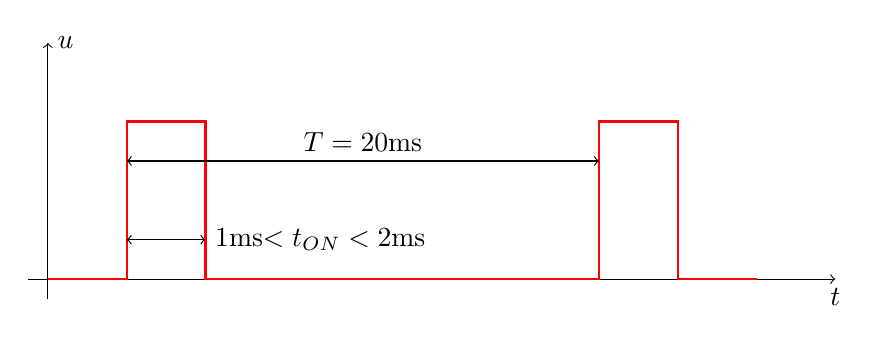
\begin{tikzpicture}
		% Achsen
		\draw[->] (-0.25,0) -- (10,0) node[anchor=north] {$t$};
		\draw[->] (0,-0.25) -- (0,3) node[anchor=west] {$u$};
		% Signal
		\draw[-,red,thick] (0,0) -- (1,0) -- (1,2) -- (2,2) -- 
			(2,0) -- (7,0) -- (7,2) -- (8,2) -- (8,0) -- (9,0);
		% Zeiten
		\draw[<->] (1,1.5) -- (7,1.5) node[midway, above] {$T=20$ms};
		\draw[<->] (1,0.5) -- (2,0.5) node[right] {$1$ms$<t_{ON}<2$ms};
	\end{tikzpicture}
	\caption{Signalverlauf eines typischen Modellbau-PWM Signals}
	\label{fig:rc-pwm}
\end{figure}
\fi

Der Einsatz von Modellbausteuerungen für BLDC-Motoren erfordert ein
Feedback der Drehzahl, da diese lediglich eine Steuerung darstellen. Die
Drehzahlregelung muss über eine externe Einheit erfolgen, wie etwa einen
Mikrocontroller. Solche BLDC-Steuerungen werden im Modellbau typisch als
\emph{Regler} vertrieben und sind auch für hohe Leistungen relativ günstig.

\ifSTANDALONE
\subsection{Konzeptbeschreibung}
\fi
\ifEMBED
\subsubsection{Konzeptbeschreibung}
\fi
Um eine Regelung der Drehzahl des BLDC-Motors zu ermöglichen, bedarf es eines
Feebacks, welches die Drehzahl wiedergibt. Dies ist mit einem
Hall-Effekt-Schalter zu realiseren. Dieser reagiert auf die Magnetfelder,
welche durch Magnete auf dem Rotationskörper gegeben sind. Aus solch einem
Aufbau resultiert ein Feeback, welches mittels Impulsen einen Segmentdurchlauf
des Rotationskörpers wiedergibt wie in der Abbildung \ref{fig:fallback-sketch}
dargestellt.
\ifSTANDALONE
\begin{figure}[h!]
	\centering
	\includegraphics[width=0.8\textwidth]{../src/Bilder/fallback_sketch_1.pdf}
	\caption{Erste Skizze des Fallback-Konzepts}
	\label{fig:fallback-sketch}
\end{figure}
\fi
Dieses Feedback wird mittels eines Mikrocontrollers ausgewertet und regelt
damit den Input der Steuerung mittels des PWM-Signals bzw. der Impulsdauer.
Das Einlesen einer Flanke, die Zeitmessung bis zur nächsten Flanke und die
Stellung eines PWM-Signals sind Tasks, welche übliche Mikrocontroller direkt
durch ihre Peripherie-Module ausführen können. Dies ermöglicht eine einfache
Adaption in ein bestehendes Modell, denn es werden lediglich zwei Timer-IO
für dieses Fallback verwendet. Je nach Mikrocontroller ist ein Pegelwandler
notwendig für die PWM-Signale.

	\newpage
	\ifSTANDALONE
\section{Encoder \& Drehzahlgeber}
\fi
\ifEMBED
\subsection{Encoder \& Drehzahlgeber}
\fi

Die vorgesehenen Motorfunktionen verlangen lediglich beim Brushlessmotor
nach einem Feedback über die Rotation des Motors, da der Schrittmotor
definiert und feingranuliert betrieben wird und der Gleichstrommotor
keinerlei Ansprüche stellt weder an Drehzahl noch an Position.

Encoder sind relativ teuer und der Einsatz des Brushlessmotors verlangt
lediglich nach einem Feedback zur Rotation bzw. Winkelgeschwindigkeit.
Die absolute oder relative Position ist für die Anwendung nicht von
Bedeutung. Somit lässt sich ein einfaches Feedback vorsehen für die
Regelung der Drehzahl mittels optischer oder magnetischer Elemente.
\ifSTANDALONE
\begin{figure}[h!]
	\centering
	\begin{tikzpicture}
		% Koordinaten
		\draw[->] (-0.5, 0) -- (8, 0) node[anchor=north] {$t$};
		\draw[->] (0, -1.5) -- (0, 3) node[anchor=east] {$u,\varphi$};
		% Rotation
		\draw[blue] (0,0) sin (1,1) cos (2,0) sin (3,-1) cos (4,0)
			sin (5,1) cos (6,0) sin (7,-1)
			node[right] {$\varphi$};
		% Signal
		\draw[-, thick, red]
			(0,0) -- (0.8,0) -- (0.8,2) -- (1.2,2) -- (1.2,0) -- 
			(4.8,0) -- (4.8,2) -- (5.2,2) -- (5.2,0) -- (7.5,0);
		% Messung
		\draw[<->] (0.8,1.5) -- (4.8,1.5) node[midway, above] {$t_{r}$};
	\end{tikzpicture}
	\caption{Vereinfachtes Puls-Feedback eines Hall-Effekt-Scahlters}
	\label{fig:hall-effekt-schalter}
\end{figure}
\fi
\ifEMBED
\begin{figure}[h!]
	\centering
	\begin{tikzpicture}
		% Koordinaten
		\draw[->] (-0.5, 0) -- (8, 0) node[anchor=north] {$t$};
		\draw[->] (0, -1.5) -- (0, 3) node[anchor=east] {$u,\varphi$};
		% Rotation
		\draw[blue] (0,0) sin (1,1) cos (2,0) sin (3,-1) cos (4,0)
			sin (5,1) cos (6,0) sin (7,-1)
			node[right] {$\varphi$};
		% Signal
		\draw[-, thick, red]
			(0,0) -- (0.8,0) -- (0.8,2) -- (1.2,2) -- (1.2,0) -- 
			(4.8,0) -- (4.8,2) -- (5.2,2) -- (5.2,0) -- (7.5,0);
		% Messung
		\draw[<->] (0.8,1.5) -- (4.8,1.5) node[midway, above] {$t_{r}$};
	\end{tikzpicture}
	\caption{Vereinfachtes Puls-Feedback eines Hall-Effekt-Scahlters}
	\label{fig:hall-effekt-schalter}
\end{figure}
\fi
Als optisches Messisnturment kann eine Lichtschranke mit 
Reflexionsstriefen oder Löchern eingesetzt werden. Diese verlangen
nur nach einer geringfügigen Modifikation des Rotierenden Körpers und
sind relativ günstig. Optische Messtechnik hat den Nachteil, dass
Störungen relativ leicht in die Messung einfliessen können, was fatale
Folgen für die Regelung hat. Magnetische Messinstrumente sind gegenüber
Störungen deutlich resistenter, da hierfür starke Magnetfelder benötigt
werden, welche so nicht einfach auftreten. Der Einsatz solcher Messtechnik
verlangt jedoch nach einer Modifikaiton der Mechanik, da Magnete in den
rotierenden Körper einebaut werden müssen. Dies birgt ein gewisses
Risiko für mechanische Unwucht des Rotationskörpers.

\ifSTANDALONE
\subsection{Magnetischer Drehzahlgeber}
\fi
\ifEMBED
\subsubsection{Magnetischer Drehzahlgeber}
\fi
Um einen eigenen magnetischen Drehzahlgeber zu erstellen wird ein
sog. Hall-Effekt-Schalter eingesetzt. Dieser reagiert mit seinem Ausgang
auf ein auftretendes Magnetfeld. Das Gegenstück zum Hall-Effekt-Schalter
ist ein Magnet, welcher in das rotierende Objekt eingebaut wird. Aus 
mechanischen Gründen, wie etwa der Unwucht, werden typisch 2 Magnete
oder ein Vielfaches davon in den rotierenden Körper eingebaut.

Bei der Rotation des Körpers entstehen durch das Vorbeigehen der Magnete
am Hall-Effekt-Schalter Impulse. Aus diesen Impulsen lässt sich mittels einer
Zeitmessung direkt die Drehzahl bestimmen. Die Abbildung 
\ref{fig:hall-effekt-schalter} illustriert das Prinzip anhand eines
Beispiels mit einem Magneten am Rotationskörper.
%
\ifSTANDALONE
\begin{figure}[h!]
	\centering
	\includegraphics[width=0.75\textwidth]{\BrushlessPath/Bilder/AH180N_functional.png}
	\caption{Funktionelles Blockschaltbild des Hall-Effekt-Scahlters AH180N}
	\label{fig:AH180N_functional}
\end{figure}
\fi
%
\ifEMBED
\begin{figure}[h!]
	\centering
	\includegraphics[width=0.75\textwidth]{\BrushlessPath/Bilder/AH180N_functional.png}
	\caption{Funktionelles Blockschaltbild des Hall-Effekt-Scahlters AH180N}
	\label{fig:AH180N_functional}
\end{figure}
\fi
%
Ein solches Verfahren lohnt sich bei schnellen Winkelgeschwindigkeiten
und ist für diesen Anwendungsfall sehr effizient. Zugehörige
Hall-Effekt-Schalter lassen sich einfach montieren und sind gegen Störungen
sehr robust. Ein mögliches Modell für einen Hall-Effekt-Schalter ist der
AH180N. Dieser bietet einen Open-Drain Ausgang welcher somit logische Pegel
liefert (siehe Abbildung \ref{fig:AH180N_functional}). Interessant ist diese
Art von Drehzahl-Geber insbesondere durch ihren geringen Preis, denn solche
Hall-Effekt-Schalter wie der AH180N befinden
sich im Preissegment < 1 CHF.

	\clearpage
	\setlength\bibitemsep{1.5\itemsep}
\nocite{*}
\bibliography{\BIBLIOGRAPHY}
\bibliographystyle{apacite}

	\listoffigures
	\listoftables
\end{document}
